\chapter{Methods and Procedure}
\label{chapter:methods}

In Figure \ref{fig:image}, the processing pipeline for this project is shown.

\begin{figure}[h!]
    \centering
    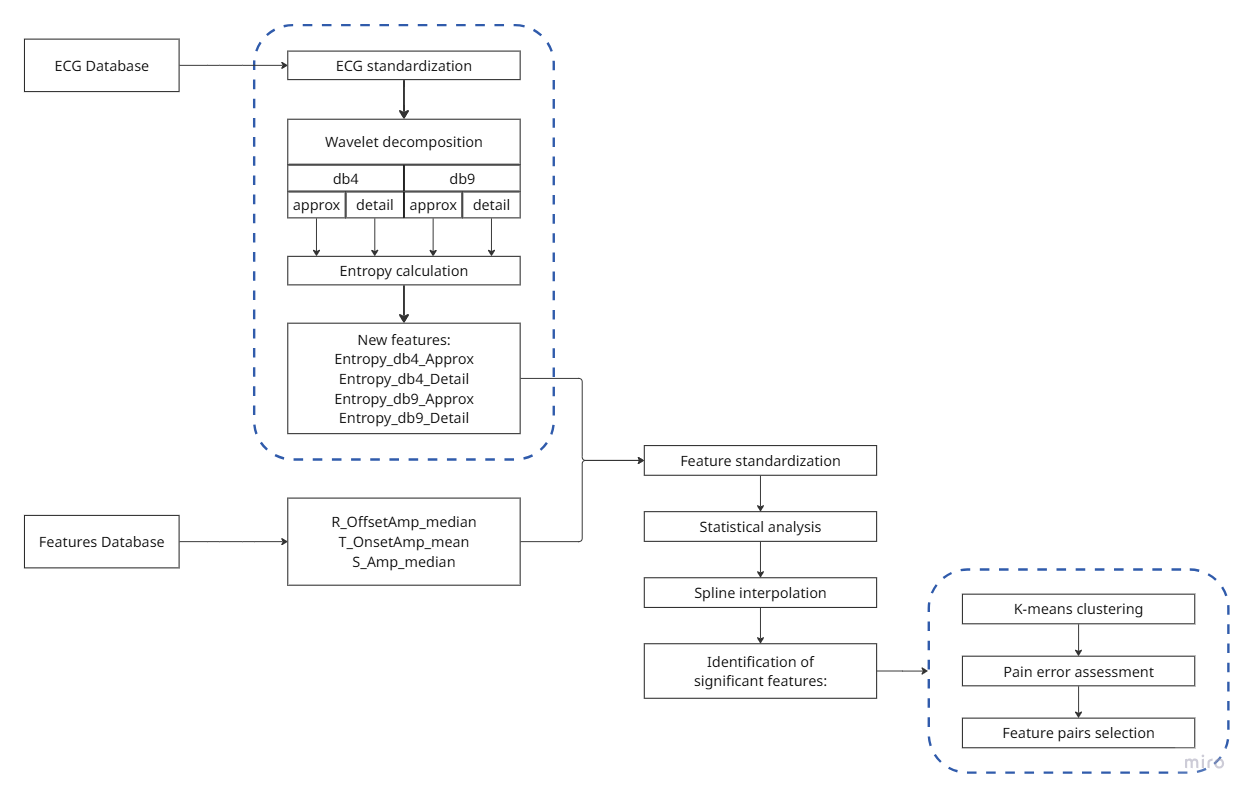
\includegraphics[width=1.0\textwidth]{image.png}
    \caption{Processing pipeline.}
    \label{fig:image}
\end{figure}

\section{Database Acquisition}
In this project, two databases were used: one has data from an \ac{ecg} signal while the other contains features extracted from that \ac{ecg}, as described in the article by Alves et al \cite{Alves2024}.

The data collection protocol followed a structured sequence designed to elicit and record both emotional and pain-related responses. It began with a 5-minute baseline period, during which participants remained seated in a relaxed position without any external stimuli. During this time, only physiological signals were recorded to establish a baseline.
Subsequently, participants watched a 10-minute video, composed of excerpts from comedy, horror, or documentary films, aimed at inducing positive, negative, or neutral emotional states, respectively. This was immediately followed by a second 5-minute stimulus-free period, allowing for recovery and stabilization of physiological responses.
Next, participants underwent a \ac{cpt}, in which they immersed their non-dominant hand in a tank of cold water maintained at 7 ± 1°C. This procedure aimed to induce pain, and participants reported their experience using the \ac{nps} at four key time points: (1) before immersing the hand, (2) at the moment pain was first perceived (Pain Threshold), (3) when the pain became unbearable (Pain Tolerance), and (4) three minutes after hand removal. The \ac{cpt} phase concluded either when the participant reached their pain tolerance or after a maximum of 2 minutes, whichever occurred first.
Finally, the protocol concluded with a third 5-minute period without stimuli, serving as a rest phase to observe post-task physiological responses. 
This process is depicted in Figure \ref{fig:database}. 


\begin{figure}[h!]
    \centering
    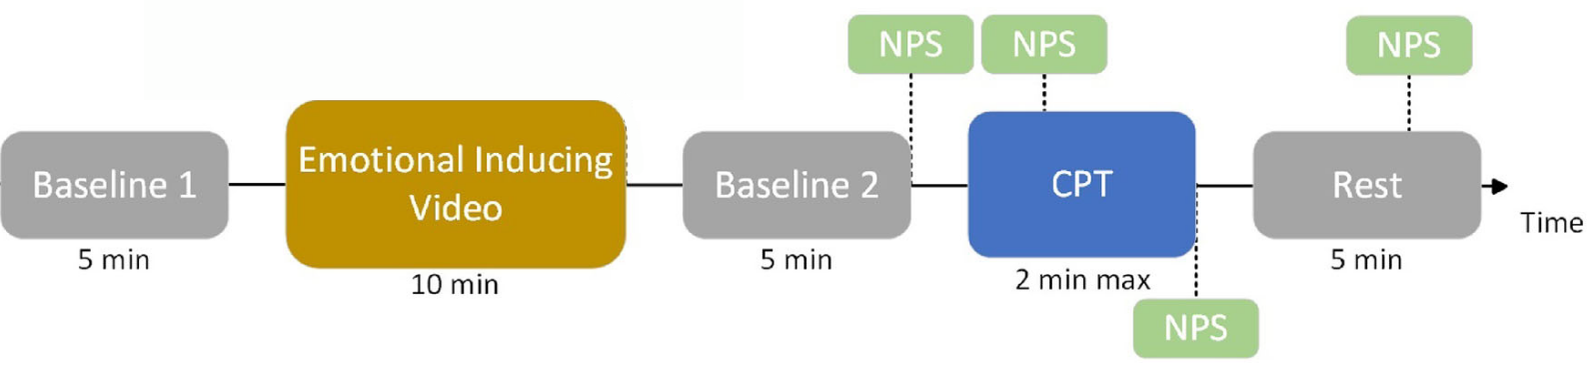
\includegraphics[width=1.0\textwidth]{database.png}
    \caption{Scheme of the protocol applied to obtain the database. (Adapted from \cite{Alves2024})}
    \label{fig:database}
\end{figure}

During the study, three physiological signals were recorded: \ac{ecg}, \ac{eda}, and \ac{emg}, with \ac{emg} signals collected specifically from the trapezius and triceps muscles. Among these, the \ac{ecg} data were stored in a dedicated database, which was subsequently used in the present project.
From the \ac{ecg} signals, several time series were extracted, including \ac{hr}, amplitude of wave peaks, amplitude of onsets and offsets, and the intervals between consecutive onsets, offsets, and peaks. These features were computed using 10-second sliding windows with 50\% overlap.
For each window, a set of statistical metrics—namely the mean, median, and variance—was calculated, resulting in a total of 237 features. These were compiled into a features database, which was also employed in the current project. 





\section{Feature Extraction}
Four of all the extrated features revealed to be more related to pain assessment, by the use of a Random Forest classifier as the estimator and
the median as the threshold \cite{Alves2024}. So, under the scope of this project, the median of the R wave offset amplitude, the median of the T wave onset amplitude, and the mean and median of the S wave peak amplitude were used as a base for subsequent analysis.
Considering that the previously described features are examples of the state of the art features in \ac{ecg} analysis, and knowing that the pain quantification or identification is still an open area, this work wants to understand and find out other possible features that may describe the pain process. So, to accomplish such goal, an exploratory analysis to the collected \ac{ecg} was performed.

% In the aforementioned article, the features of the ECG that can be used to best describe pain are defined.
% Hence, the top four features were selected for analysis, namely, the median of the R wave offset amplitude, the median of the T wave onset amplitude, and the mean and median of the S wave peak amplitude.

% To enhance this research, new features were sought out. For this reason, analysis of the ECG database itself was deemed necessary. 


\subsection{\ac{ecg} Data Exploration}
When looking at the time series of the signal, in Figure \ref{fig:ecg}, it's noticeable that the range of amplitudes of the QRS complex is way bigger than that of the P and T waves.
To tackle this, the \ac{ecg} signal was standardized according to equation \ref{eq:1}, where X is the original \ac{ecg}, $\mu$ is the mean, $\sigma$ is the standard deviation and Z is the standardized signal, which has mean zero and standard deviation one. 
This means the range of values is the same for all participants, reducing the intervariability that is induced by the initial state of the participant, since it is an uncontrolled variable.

\begin{equation} \label{eq:1}
Z = \frac{X-\mu}{\sigma}
\end{equation}

% \begin{figure}[h!]
%     \centering
%     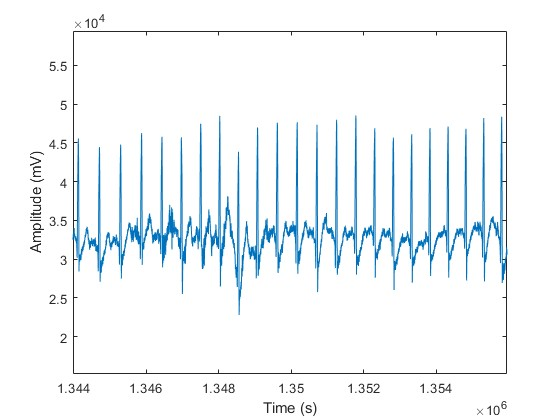
\includegraphics[width=0.9\textwidth]{ecg.jpg}
%     \caption{Section of the ECG signal of a participant.}
%     \label{fig:ecg}
% \end{figure}

\begin{figure}[htbp]
    \centering
    \begin{minipage}{0.45\textwidth}
        \centering
        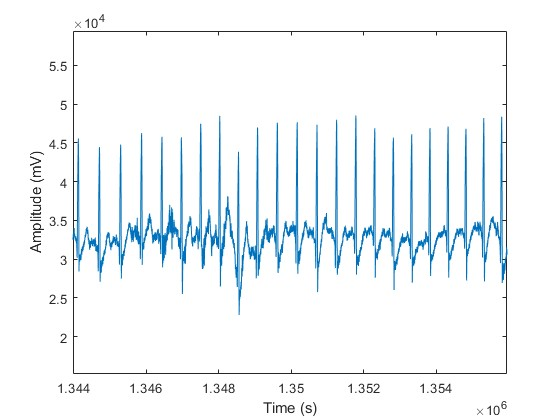
\includegraphics[width=6.8cm]{ecg}
        \caption{Section of the \ac{ecg} signal of a participant.}
        \label{fig:ecg}
    \end{minipage}
    \hfill
    \begin{minipage}{0.45\textwidth}
        \centering
        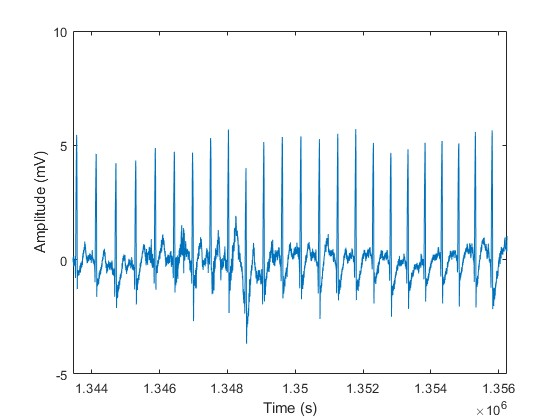
\includegraphics[width=6.8cm]{normalized ecg}
        \caption{Section of the standardized \ac{ecg} signal of a participant.}
        \label{fig:normalized_ecg}
    \end{minipage}
\end{figure}

Once the signal was standardized, fluctuations were noticed in the time series.
By removing high frequencies from the signal, by filtering for example, these would be alleviated.
However, there could be information related to pain associated to those frequencies.
A solution to these problems is to decompose the signal in wavelets, using \ac{dwt}. 

Wavelets are built upon basic functions that preserve properties of localization in both frequency and time domains, resembling short wave-like signals. The computation of a \ac{dwt} is primarily based on the employment of low-pass and high-pass filters with different cutoff frequencies to process signals in various frequency bands. This process leads to the decomposition of the signal into approximation and detail components. The approximation component represents the low-frequency content (signal energy), while the detail component captures the high-frequency content associated with short pulses, sudden changes, and noise. The amount of information is changed by filtering, and the scale is changed by decimation and interpolation. Decimation corresponds to lowering the sampling rate. 

There are many wavelet families, that differ from each other in the format of the approximation wave, but the selection of one should consider the characteristics of the signal and the decomposition level must be chosen accordingly. For this project, two types of wavelet were chosen, according two specific criteria: one's format should be similar to that of the \ac{ecg} wave, complementing the remaining features in gathering whether the QRS complex is relevant to describe pain, and the other should have a higher frequency, to understand if there's important information associated with the fluctuations of the signal, while still maintaining its smoothness.
Accordingly, Daubechies-4 ('db4') and Daubechies-9 ('db9') were chosen, which waveforms can be seen in Figure \ref{fig:waveform}. 

\begin{figure}[h!]
    \centering
    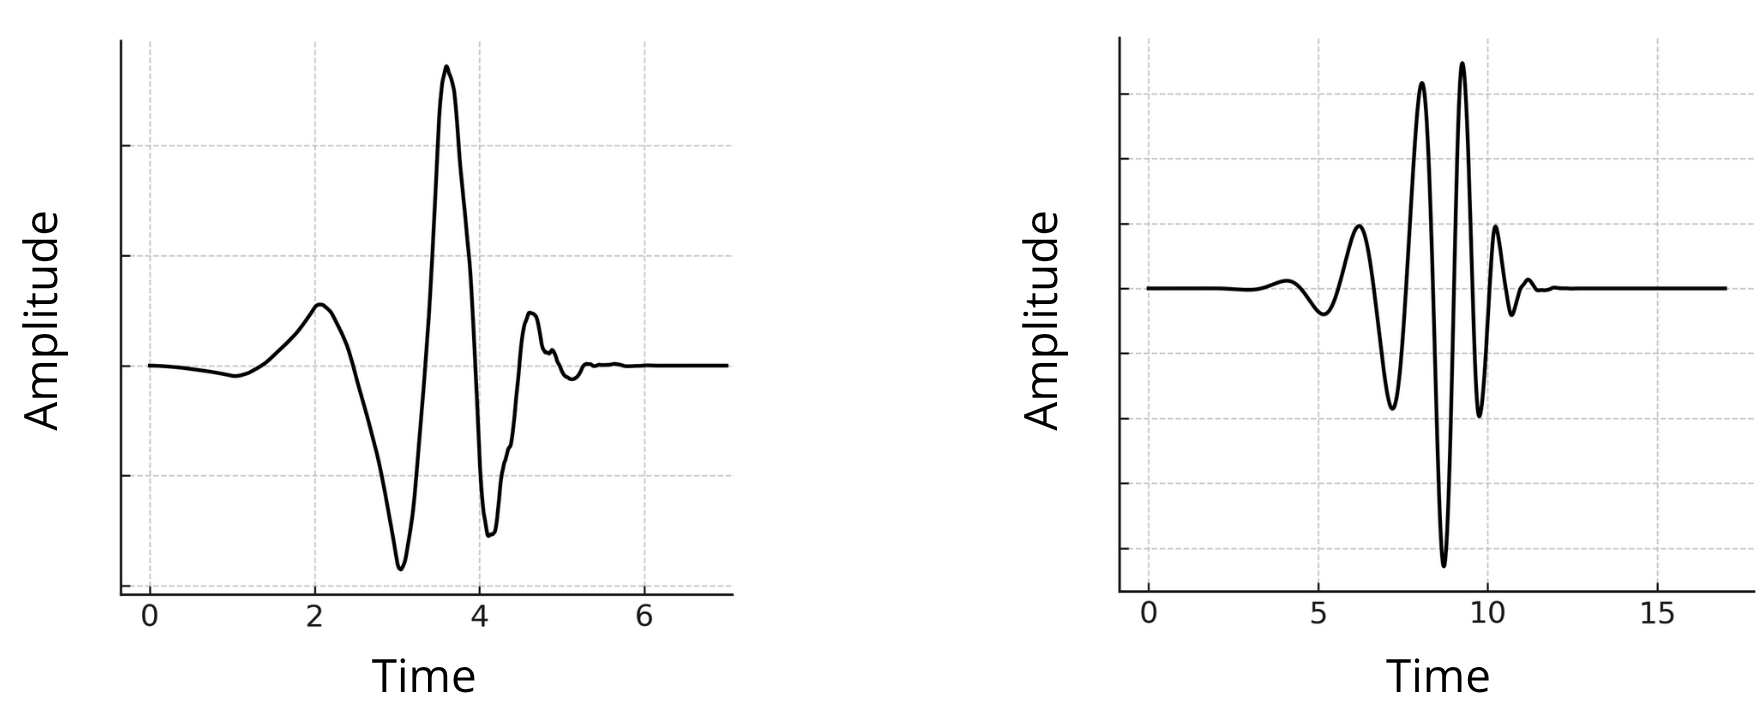
\includegraphics[width=0.7\textwidth]{wavelet_db4_db9.png}
    \caption{Daubechies-4 and Daubechies-9 Waveform.}
    \label{fig:waveform}
\end{figure}



Regarding the number of levels of decomposition, as can be seen in Figure \ref{fig:wavelets2}, when there are two levels the R peak is noticeable in the first detail, which is not something this project means to highlight.
Therefore, only one level of decomposition was applied.

\begin{figure}[h!]
    \centering
    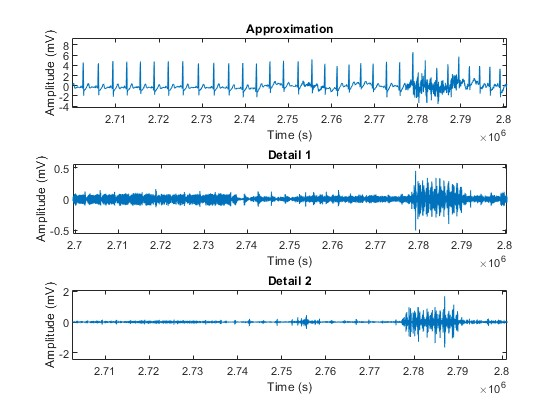
\includegraphics[width=0.8\textwidth]{wavelets 2.jpg}
    \caption{Daubechies-4 Wavelet Decomposition - level 2.}
    \label{fig:wavelets2}
\end{figure}


\subsection{Entropy Calculation}
Entropy quantifies the disorder in time series data. Due to this, features associated with it have been used in the analysis of physiological signals \cite{Koh2022}. Since this quantity might be affected in the \ac{ecg} when someone experiences pain, it was calculated for the approximation and detail components of the resulting wavelets. In order to keep consistency with the other features, a same sized window was used, that is, 10 seconds with 50\% overlap. %Since the aim of the selected features is to classify pain, which will be done by comparing the pain induction period with a baseline, 

There are various types of entropy. To select one, a research was executed on the tool Scopus using the key words entropy, ecg, signal, pain, and classification. Only four articles were found, but two of them weren't focused on pain description. Due to this, only the remaining two were analysed. Maity and Jana \cite{Maity2023} analysed four types of entropy applied to wavelets using a \ac{rf} model, while Adjei et al \cite{Adjei2017} calculated permutation entropy using Shannon entropy. These articles show that there isn't a lot of research that uses entropy for pain description, so the type of entropy was chosen based on the aim of the selected features, which is to evaluate if there are signal transitions in the presence of pain. Due to this, a \ac{tde} was implemented. The amplitude range of the signal was segmented into 100 non-overlapping and successive partitions. For each of these, the probability $P_i$ was determined by computing the ratio between the number of signal samples in that interval, and the total number of samples in the window. The entropy was then calculated using Equation \ref{eq:2}, where M equals the number of partitions \cite{Ferreira2017}. 

\begin{equation} \label{eq:2}
\ac{tde}=-\sum_{i=1}^{M}P_ilog(P_i)
\end{equation}

Although this method of computing entropy uses fixed partitioning, an adaptative partitioning alternative was also calculated, where the amplitude range that was segmented was the window's, instead of the signal's. The results for both of these entropies is displayed in Figure \ref{fig:entropies}. However, these were very similar, so only the fixed partitioning method was used, since it displays broader changes in amplitude, as can be seen in Figure \ref{fig:entropies} (right). 

\begin{figure}[h!]
    \centering
    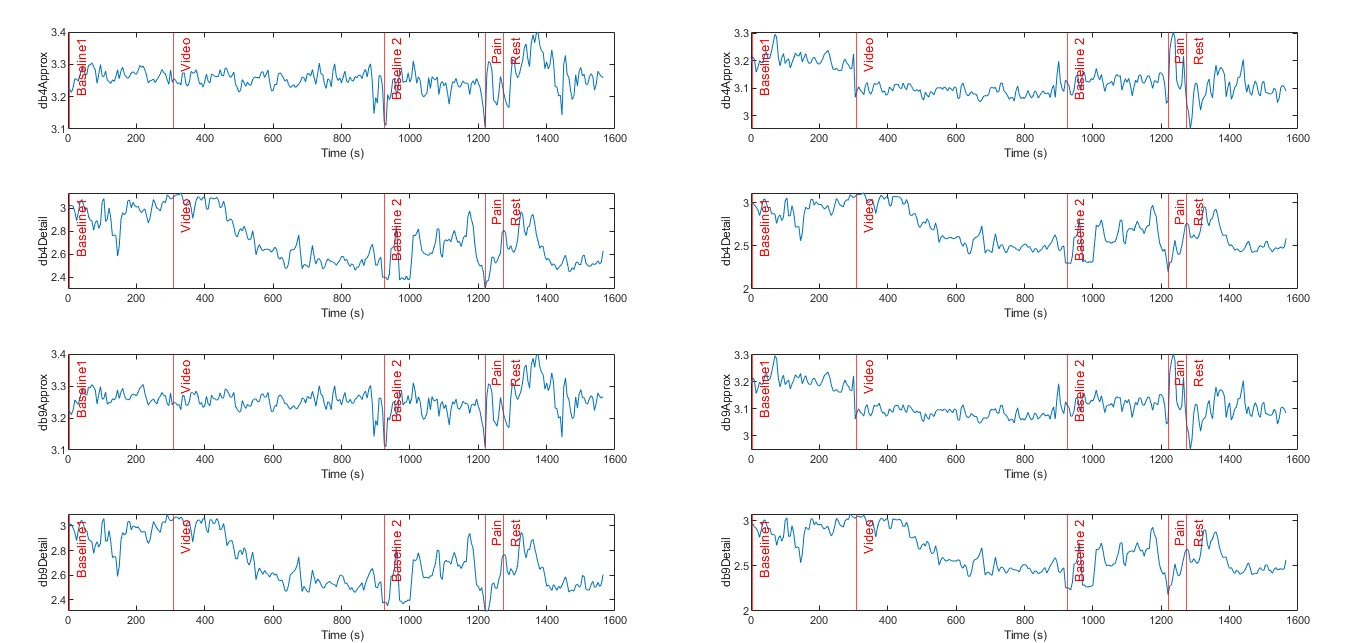
\includegraphics[width=1\textwidth]{entropy comparisons.jpg}
    \caption{Graph of the entropy computed for the approximation and detail components of the wavelets, using adaptative (left) and fixed (right) partitioning.}
    \label{fig:entropies}
\end{figure}



\section{Data Analysis}
To do the optimal processing of the features, fifteen participants were selected at random. After standardizing the features, so that they're comparable with each other, graphics of the time series of the features were plotted for each participant. An example can be seen in Figure \ref{fig:featurestimeseries}, in which a clear change can be seen when the participant dips their hand in water, feeling pain. Since the timeseries of the mean and median of the S wave amplitude were so similar, it was decided that only the median would be analysed.


\begin{figure}[htbp]
    \centering
    \begin{subfigure}{\linewidth}
        \centering
        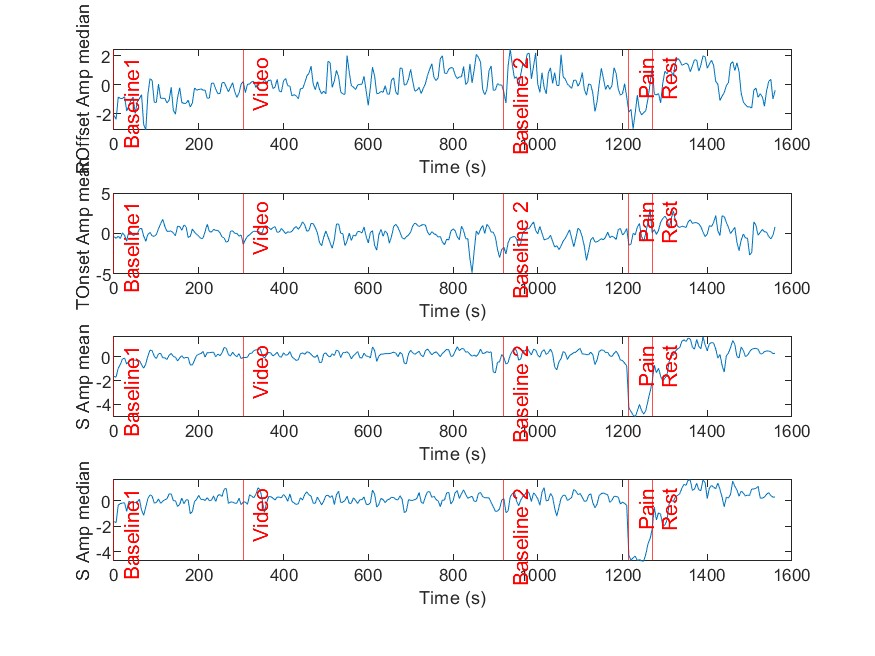
\includegraphics[width=\textwidth]{orig_part5.jpg}
    \end{subfigure}
    
    \vspace{0.1em} % adjust spacing between the two graphs
    
    \begin{subfigure}{\linewidth}
        \centering
        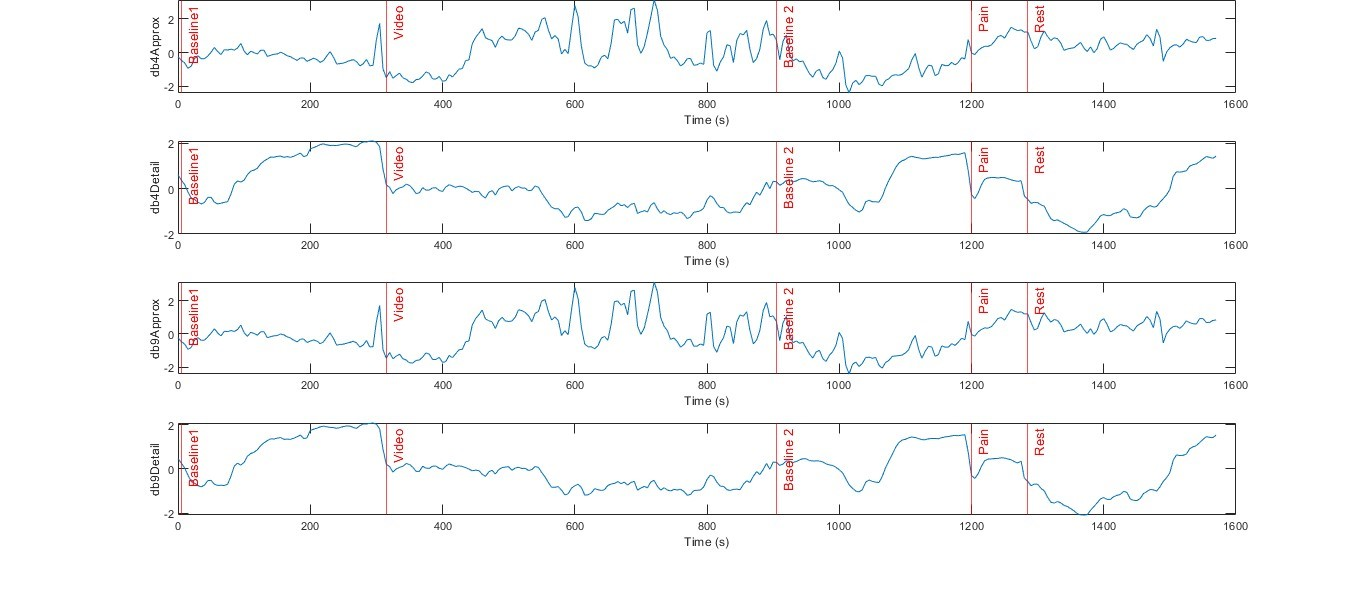
\includegraphics[width=\textwidth]{entropy_part5.jpg}
    \end{subfigure}
    
    \caption{Standardized features' time series.}
    \label{fig:featurestimeseries}
\end{figure}


Subsequently, a statistical analysis of the participants' features was conducted using histograms, as illustrated in Figure \ref{fig:histogram}. The histograms revealed that the distributions of the features deviate from normality, justifying the use of the median and \ac{iqr} as measures of central tendency and dispersion, respectively.
These values were computed for each feature and considered as derived features that will integrate the analysis.

\begin{figure}[h!]
    \centering
    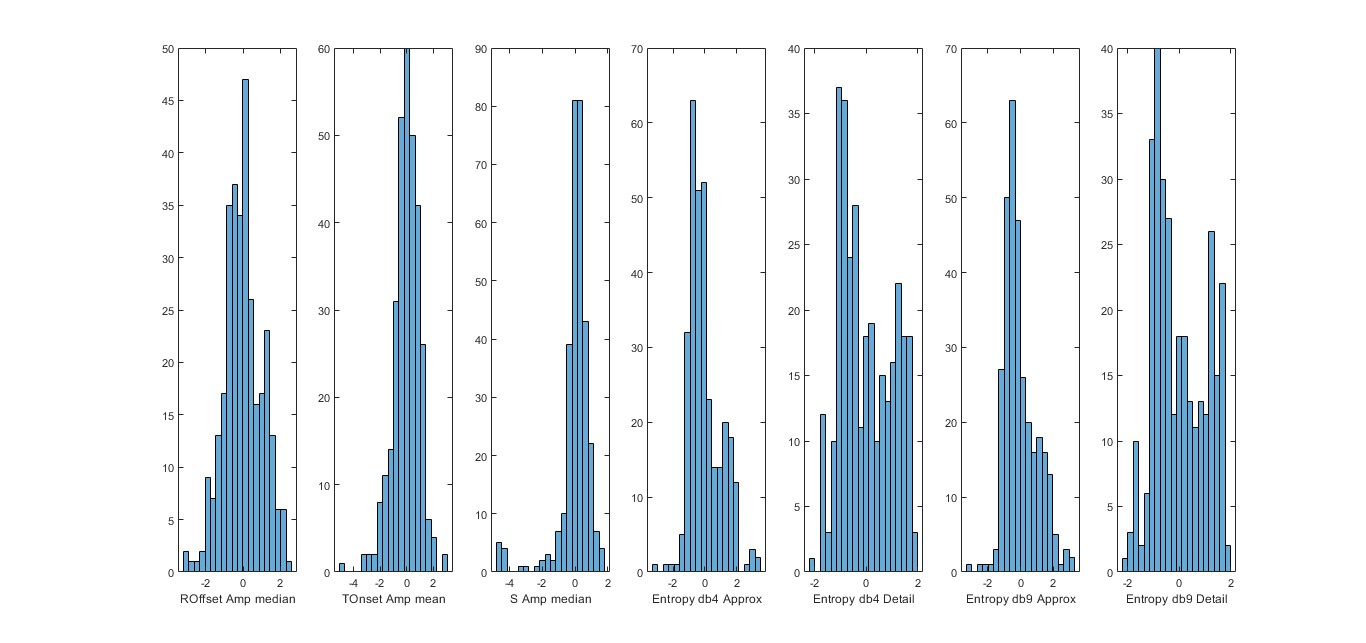
\includegraphics[width=\textwidth]{histogram.jpg}
    \caption{Histograms of the features.}
    \label{fig:histogram}
\end{figure}



The goal of this project is to select features that distinguish pain from no pain. To do this, it's important to guarantee the synchronization between segments, so that they're comparable. To accomplish this goal, spline interpolation was done in each step, conducing to equalize the number of points to a 60 seconds intervals. The result of this method is portrayed in Figure \ref{fig:normalizedfeatures}. 

\begin{figure}[h!]
    \centering
    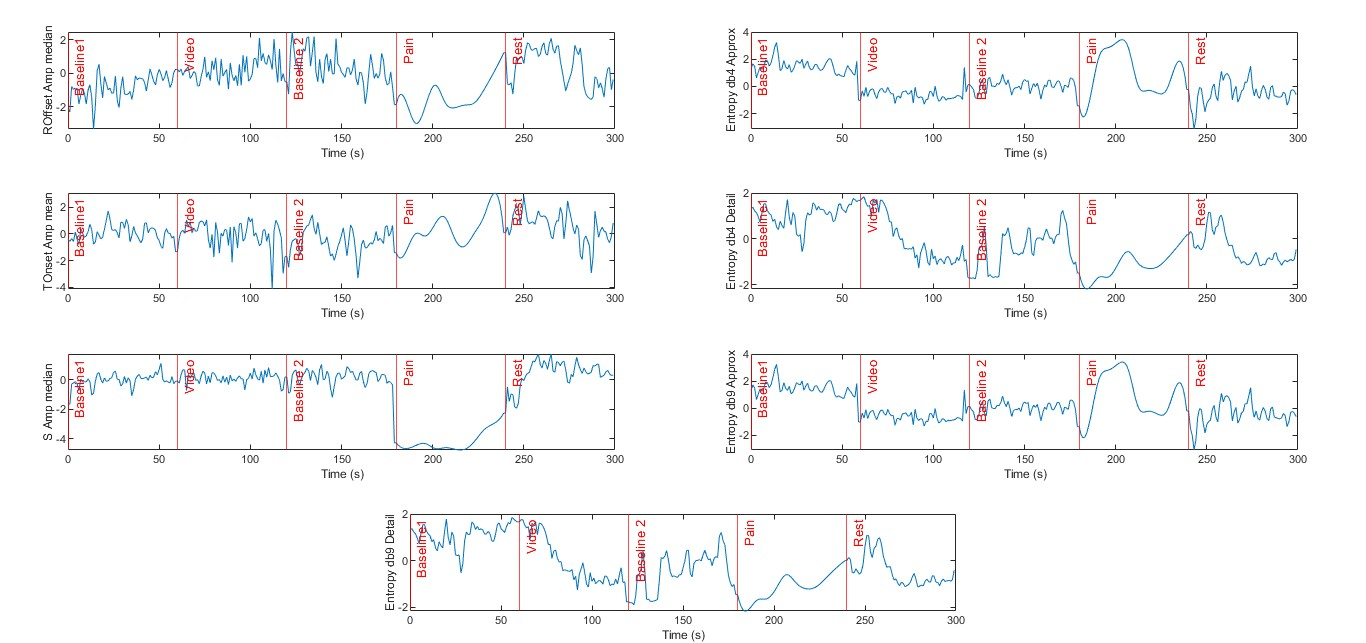
\includegraphics[width=\textwidth]{normalized features.jpg}
    \caption{Features normalized in time after interpolation.}
    \label{fig:normalizedfeatures}
\end{figure}

The features that will be analysed in this project are shown in Table \ref{table:features}. These have been computed using the median and \ac{iqr} of the extracted features for each step of the protocol, as mentioned before. 

(Em vez disto, colocar tabela com descrição de features de um participante?)



\begin{table}[h]
    \captionsetup{justification=raggedright, singlelinecheck=false}
    \caption{Features for pain classification after data preparation procedures.}
    \renewcommand{\arraystretch}{1.2}

    \begingroup
    \hyphenpenalty=10000
    \exhyphenpenalty=10000
    \sloppy
    \begin{tabular}{@{}>{\RaggedRight\arraybackslash}p{4cm} >{\RaggedRight\arraybackslash}p{11cm}@{}}
        \hline
        \textbf{Feature Source} & \textbf{Features} \\
        \midrule
        ECG Peaks & [`Roffsetampmedian\_median', `Roffsetampmedian\_iqr', `Tonsetampmean\_median', `Tonsetampmean\_iqr', `Sampmedian\_median', `Sampmedian\_iqr'] \\
        [1ex]
        Wavelet Entropy & [`Entropydb4Approx\_median', `Entropydb4Approx\_iqr', `Entropydb4Detail\_median', `Entropydb4Detail\_iqr', `Entropydb9Approx\_median', `Entropydb9Approx\_iqr',  `Entropydb9Detail\_median', `Entropydb9Detail\_iqr'] \\
    \end{tabular}
    \endgroup
    \label{table:features}
\end{table}






